\section{监考怎么做(挖坑待补)}

监考的工资单价一般比其他TA工作要高,2020年左右一般是100一个小时,而且准备工作比较少,监考途中基本也就是走一走,很轻松,是不错的挣钱方法。

\subsection{如何参加}
(我还真不知道最近怎么参加,之前我都是学校给分配的。谁知道来介绍下?)

\subsection{具体怎么做}
首先学校有监考的培训,在\textit{Teaching Assistant (TA) Training Programme}为题的邮件里的Assessment and invigilation那一项就是,或者是在你的LMO里翻一下。

(挖坑待填,如果没人需要,或者学校已经不用本校生监考的话那就不写了)

\begin{figure}[H]
    \centering
    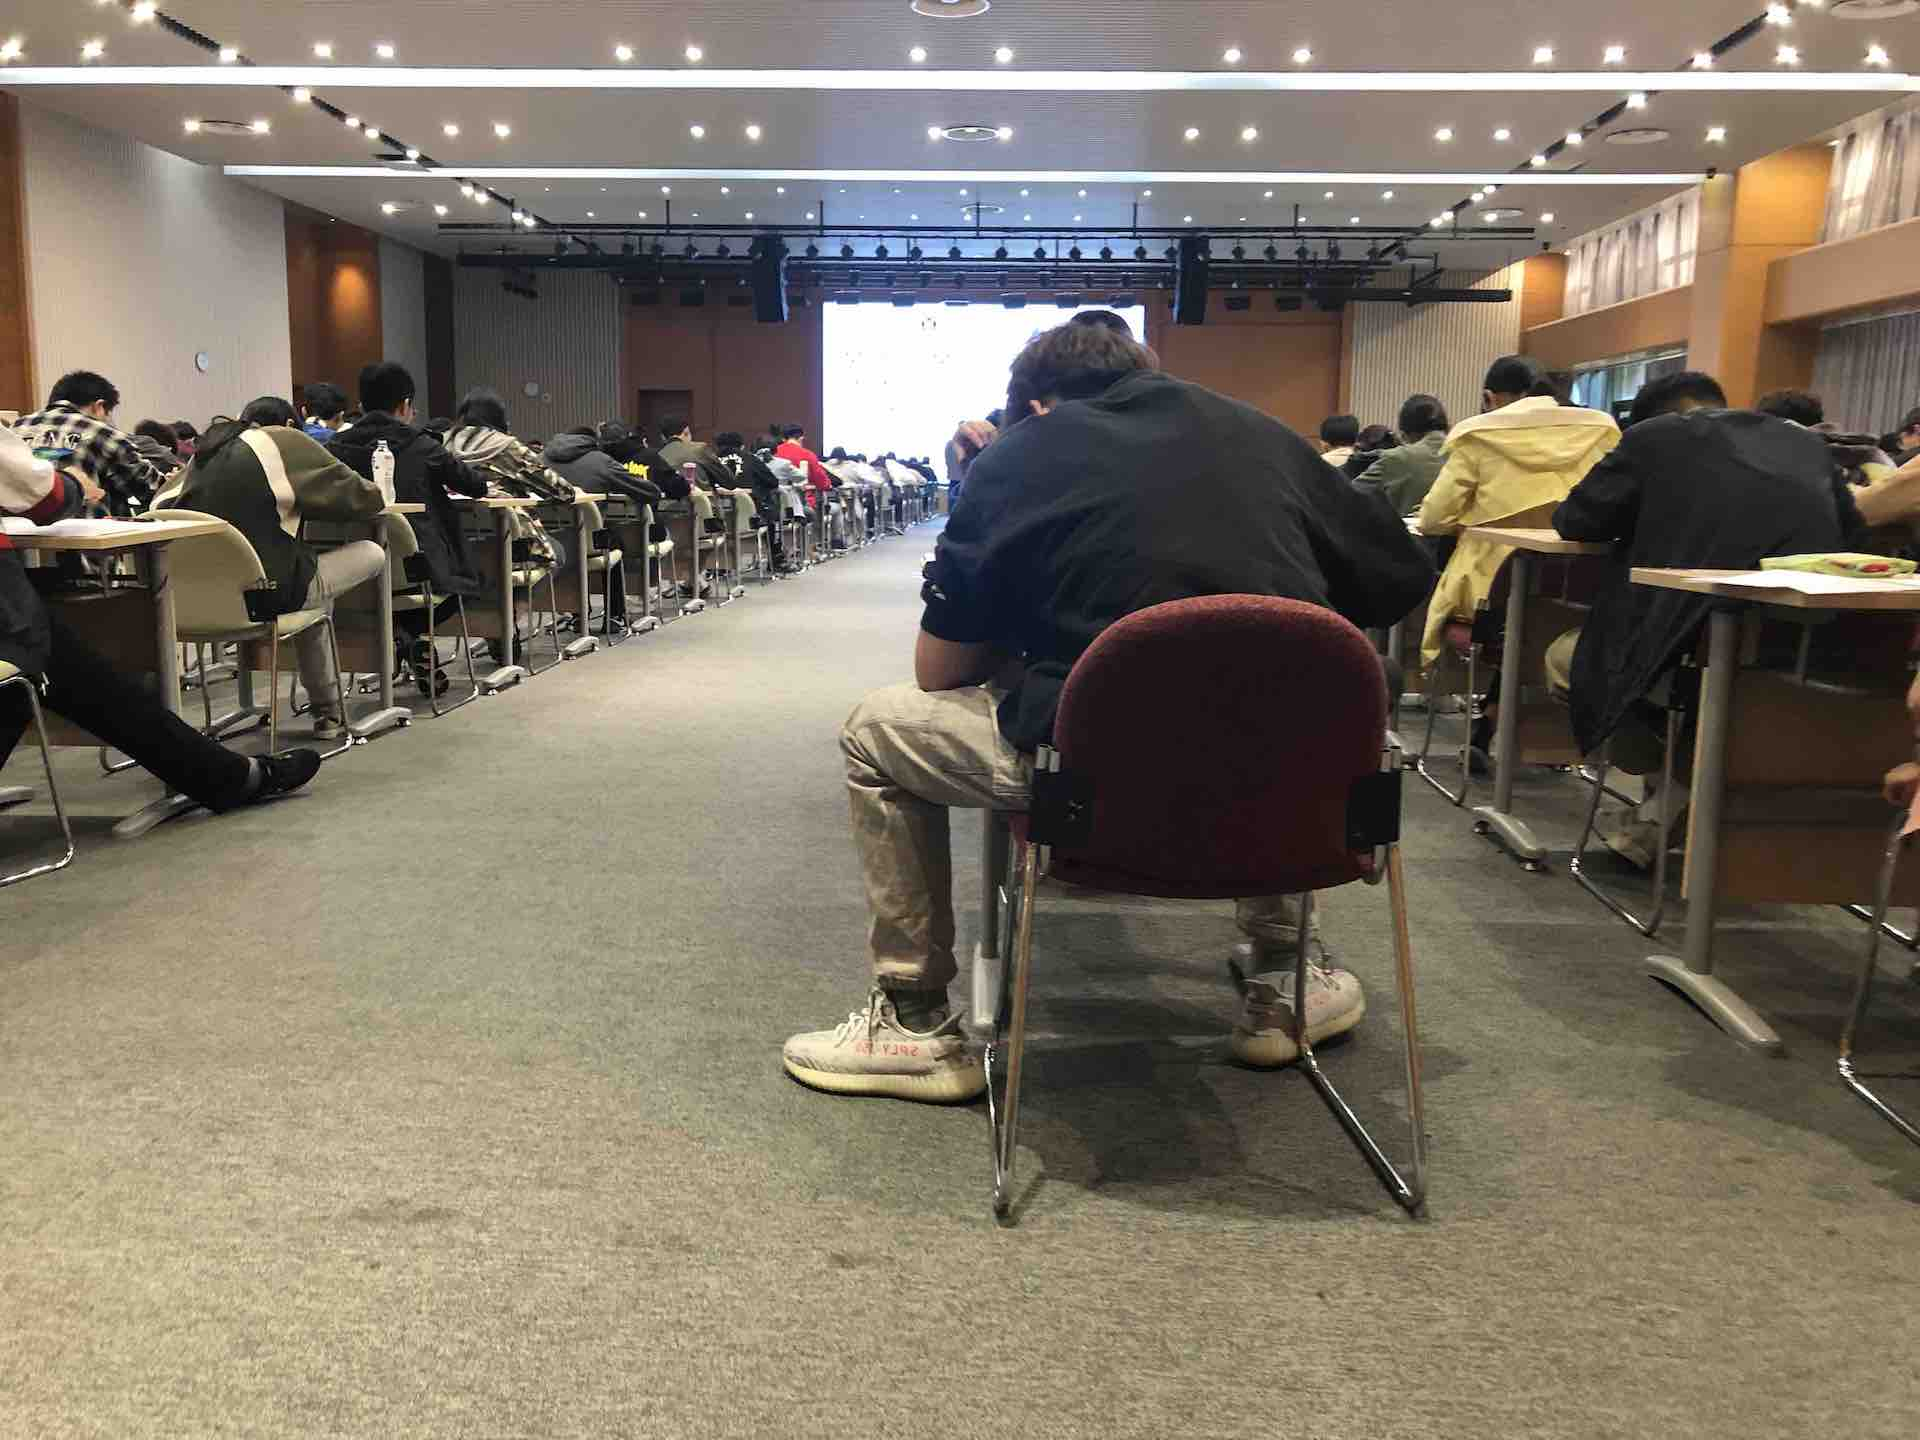
\includegraphics[width=\columnwidth]{author-folder/Kai.Wu/invigilation.jpg}
    \caption{2020年11月15日,CB楼G层某考场,监考中}
\end{figure}

\begin{flushright}
(2022年10月22日 by Kai Wu)
\end{flushright}

% \begin{figure}[H]
%     \centering
%     \includegraphics[width=0.5\columnwidth]{author-folder/Kai.Wu/}
% \end{figure}


% \usepackage[export]{adjustbox}

% \item 
% \begin{minipage}{0.3\textwidth}
%     文字
% \end{minipage}
% \begin{minipage}{0.63\textwidth}
%     \begin{figure}[H]
%         \includegraphics[width=0.4\columnwidth, right]{author-folder/Kai.Wu/}
%     \end{figure}
% \end{minipage}

% \input{author-folder/Kai.Wu/.tex}
